% $Id: template.tex 11 2007-04-03 22:25:53Z jpeltier $
\newcommand{\todo}[1]{{\bf \{TODO: {#1}\}}}
\newcommand{\projectname}{News Timeline}

\documentclass{vgtc}                          % final (conference style)
%\documentclass[review]{vgtc}                 % review
%\documentclass[widereview]{vgtc}             % wide-spaced review
%\documentclass[preprint]{vgtc}               % preprint
%\documentclass[electronic]{vgtc}             % electronic version

%% Uncomment one of the lines above depending on where your paper is
%% in the conference process. ``review'' and ``widereview'' are for review
%% submission, ``preprint'' is for pre-publication, and the final version
%% doesn't use a specific qualifier. Further, ``electronic'' includes
%% hyperreferences for more convenient online viewing.

%% Please use one of the ``review'' options in combination with the
%% assigned online id (see below) ONLY if your paper uses a double blind
%% review process. Some conferences, like IEEE Vis and InfoVis, have NOT
%% in the past.

%% Figures should be in CMYK or Grey scale format, otherwise, colour 
%% shifting may occur during the printing process.

%% These three lines bring in essential packages: ``mathptmx'' for Type 1 
%% typefaces, ``graphicx'' for inclusion of EPS figures. and ``times''
%% for proper handling of the times font family.

\usepackage{mathptmx}
\usepackage{graphicx}
\usepackage{times}

%% We encourage the use of mathptmx for consistent usage of times font
%% throughout the proceedings. However, if you encounter conflicts
%% with other math-related packages, you may want to disable it.

%% If you are submitting a paper to a conference for review with a double
%% blind reviewing process, please replace the value ``0'' below with your
%% OnlineID. Otherwise, you may safely leave it at ``0''.
\onlineid{0}

%% declare the category of your paper, only shown in review mode
\vgtccategory{Research}

%% allow for this line if you want the electronic option to work properly
\vgtcinsertpkg

%% In preprint mode you may define your own headline.
%\preprinttext{To appear in an IEEE VGTC sponsored conference.}

%% Paper title.

\title{\projectname: A Visual Analysis Tool for Heterogeneous Text Data}

%% This is how authors are specified in the conference style

%% Author and Affiliation (single author).
%%\author{Roy G. Biv\thanks{e-mail: roy.g.biv@aol.com}}
%%\affiliation{\scriptsize Allied Widgets Research}

%% Author and Affiliation (multiple authors with single affiliations).
%%\author{Roy G. Biv\thanks{e-mail: roy.g.biv@aol.com} %
%%\and Ed Grimley\thanks{e-mail:ed.grimley@aol.com} %
%%\and Martha Stewart\thanks{e-mail:martha.stewart@marthastewart.com}}
%%\affiliation{\scriptsize Martha Stewart Enterprises \\ Microsoft Research}

%% Author and Affiliation (multiple authors with multiple affiliations)
\author{Roy G. Biv\thanks{e-mail: roy.g.biv@aol.com}\\ %
        \scriptsize Starbucks Research %
\and Ed Grimley\thanks{e-mail:ed.grimley@aol.com}\\ %
     \scriptsize Grimley Widgets, Inc. %
\and Martha Stewart\thanks{e-mail:martha.stewart@marthastewart.com}\\ %
     \parbox{1.4in}{\scriptsize \centering Martha Stewart Enterprises \\ Microsoft Research}}

%% A teaser figure can be included as follows, but is not recommended since
%% the space is now taken up by a full width abstract.
%\teaser{
%  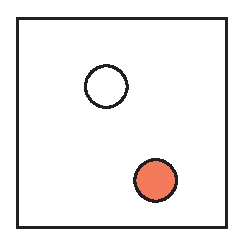
\includegraphics[width=1.5in]{sample.eps}
%  \caption{Lookit! Lookit!}
%}

%% Abstract section.
\abstract{\todo{Add the abstract after complete the summary}
} % end of abstract

%% ACM Computing Classification System (CCS). 
%% See <http://www.acm.org/class/1998/> for details.
%% The ``\CCScat'' command takes four arguments.

\CCScatlist{ 
  \CCScat{K.6.1}{Management of Computing and Information Systems}%
{Project and People Management}{Life Cycle};
  \CCScat{K.7.m}{The Computing Profession}{Miscellaneous}{Ethics}
}

%% Copyright space is enabled by default as required by guidelines.
%% It is disabled by the 'review' option or via the following command:
% \nocopyrightspace

%%%%%%%%%%%%%%%%%%%%%%%%%%%%%%%%%%%%%%%%%%%%%%%%%%%%%%%%%%%%%%%%
%%%%%%%%%%%%%%%%%%%%%% START OF THE PAPER %%%%%%%%%%%%%%%%%%%%%%
%%%%%%%%%%%%%%%%%%%%%%%%%%%%%%%%%%%%%%%%%%%%%%%%%%%%%%%%%%%%%%%%%

\begin{document}

%% The ``\maketitle'' command must be the first command after the
%% ``\begin{document}'' command. It prepares and prints the title block.

%% the only exception to this rule is the \firstsection command
\firstsection{Introduction}

\maketitle

Exploring heterogeneous data from different sources can be complicated and error pruning if not well dealt with hidden relationship between entities or possible data conflicts between materials. 
In the MC1 of VAST Challenge 2014, to extract relationship between POK and GAStech we need to extract important people from different sources of file, e.g. employee resume, email, research report, and a huge volume of news with conflicts. 
In our design of the analysis tool \projectname. \todo{Choose a better name for our tool}, we integrate different kinds of source files into a timeline-based view, providing a quick overview for user to choose important file to focus for efficiency. 
\par
In this poster, we will first introduce our design consideration of visual analysis tools for heterogeneous data and then introduce how we use these tools to analyze MC1 data to solve these problems.
%% \section{Introduction} 

%eg.\cite{kitware2003,Max:1995:OMF}

\section{Design Priciples}
Data provided in MC1 mainly includes 845 news articles, 35 resumes, employee records, email headers and some other report on both POK and Kronos. These data have the following features: 1. 


\section{Visualization Tools}
\subsection{Resume reader}
\begin{figure}[htb!]
  \centering
  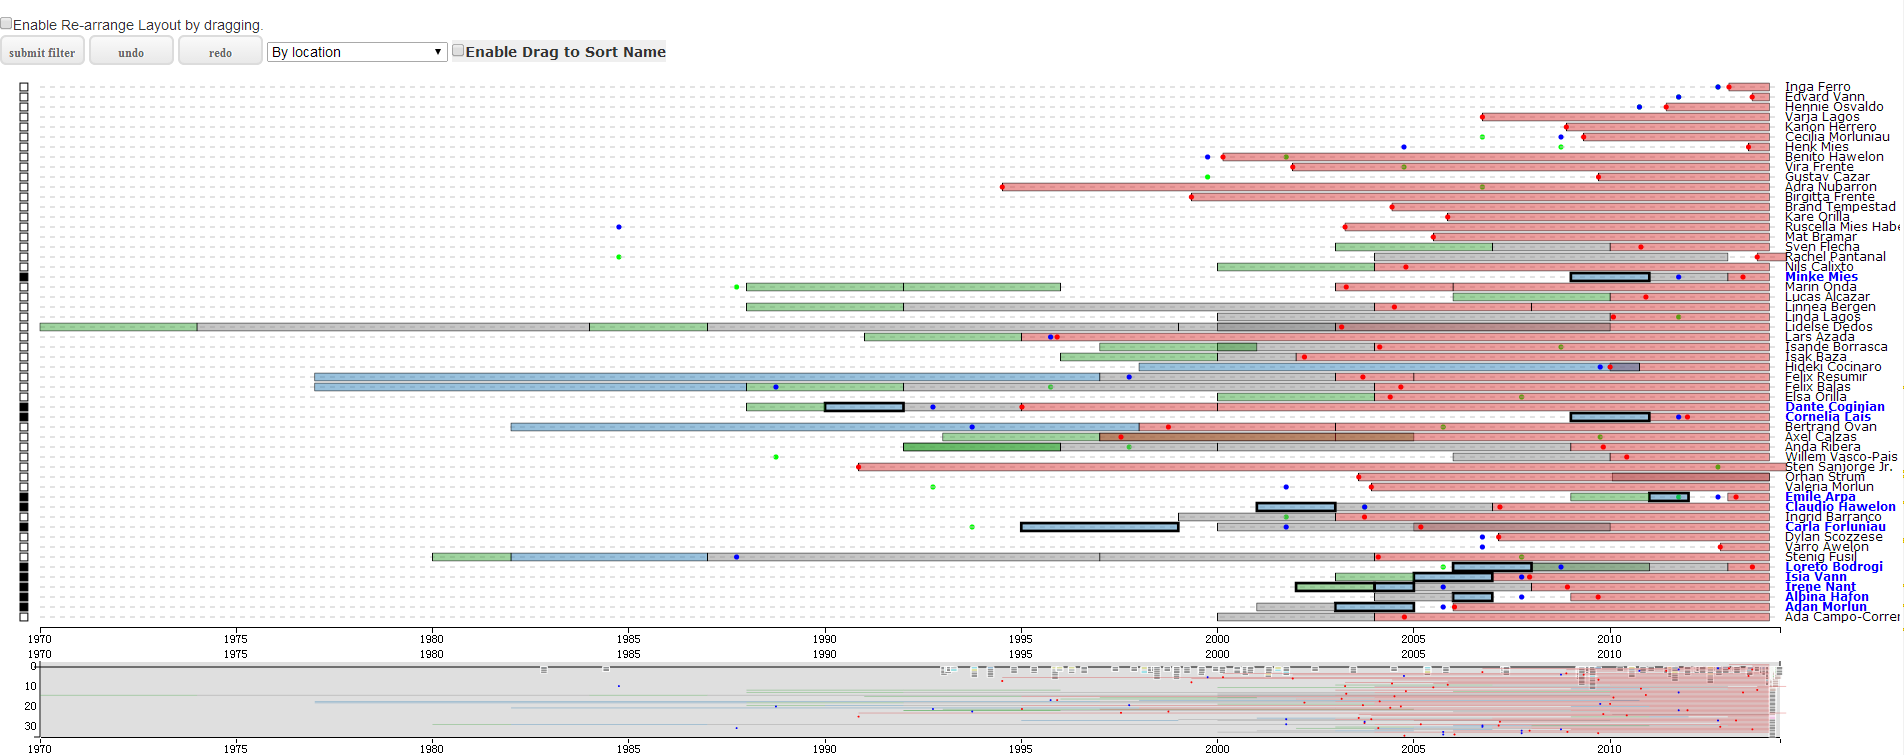
\includegraphics[width=3in]{image009.png}
  \caption{Resumer viewer}
\end{figure}
Resume reader is the fisrt paragraph.
\footnote{This is footnote}.

\subsection{News timeline}
\todo{Finish description for newstimeline.}

\subsection{Email Reader}
\todo{Finish dealing with email reader.}

\section{Data Exploration}
\todo{Describe how do we explore data sources to extract details.}

\section{Conclusion}
\todo{What do we achieve with our tool.}

%% if specified like this the section will be ommitted in review mode
\acknowledgements{
We have special thanks to Miss Dong Liu for her dedicated exploration with raw materials to inspire our design on visualization tools.
}

\bibliographystyle{abbrv}
%%use following if all content of bibtex file should be shown
%\nocite{*}
\bibliography{template}
\end{document}
